\subsection{Construcción de interfaces de usuario usando el patrón MVC}
	\subsubsection{MVC}
	El patrón \emph{Modelo-Vista-Controlador} (MVC) es una forma de construir
	interfaces de usuario (UI) que propone dividir el comportamiento de una
	aplicación en tres partes \cite{reenskaug79}:
		\begin {itemize}
		\item {\bf Modelo}
			El modelo representa nuestra percepción del mundo real. 
			Maneja el comportamiento y la información del dominio de la aplicación,
			responde a los pedidos de información sobre su estado y tiene la
			responsabilidad última de llevar a cabo el comportamiento del sistema.
			
		\item {\bf Vista}
			La vista tiene la responsabilidad de interactuar con el usuario, es la
			parte más fácil de identificar ya que es la que vemos en pantalla.
			La comunicación con el usuario es bidireccional:
			por un lado le muestra información proveniente del modelo y por el otro lado
			recibe acciones de parte del usuario, que representa internamente como eventos.
			
		\item {\bf Controlador}
			Es el intermediario entre el modelo y la vista.
			Captura los eventos emanados de ambos y coordina la interacción entre los
			dos.
	\end {itemize}
	 
	La idea principal de MVC, y que influyó a la mayoría de los frameworks de
	presentación posteriores, es la de Presentación Separada \emph{(Separated
	Presentation)} \cite{burbeck87}.
	Esto nos brinda una clara separación de responsabilidades entre interfaz,
	lógica de negocio y control. Además nos permite soportar múltiples
	presentaciones para un mismo modelo de información.
	La figura \ref{mvc} muestra las relaciones entre los tres componentes.  
	
	\begin{figure}[h]
		\centering
		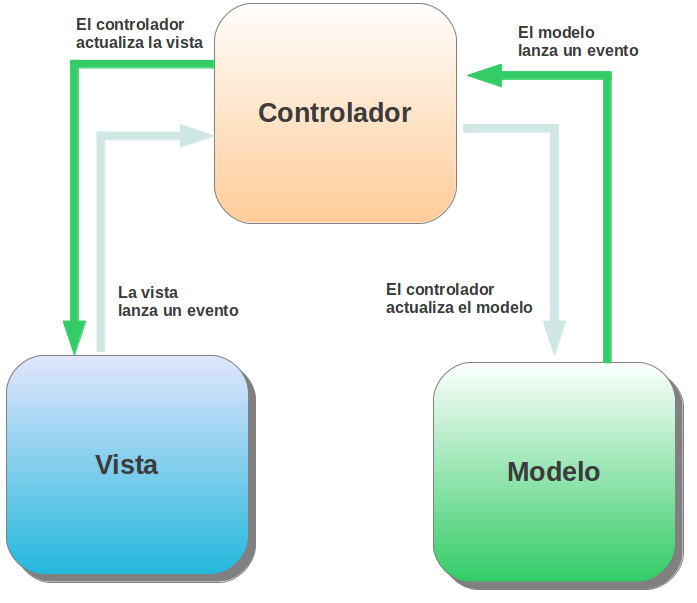
\includegraphics[width=300px, height=300px]{img/mvc} 
		\caption{Esquema MVC}
		\label{mvc}
	\end{figure}  
	
\subsubsection{Eventos}
\label{Eventos}

		Un evento es un suceso en el sistema, como una interacción del usuario con
	la máquina, o un cambio en el estado interno de un objeto.
	En un sistema orientado a eventos, existen fuentes que producen eventos y
	\emph{listeners} que se registran para ser notificados de esos eventos y poder
	actuar en consecuencia.	
	El patrón \emph{Observer} \cite{Gamma1995} es una forma común de implementar la
	idea de evento en lenguajes orientados a objetos.
	
	\begin{quote}
	
	\begin{description}
	   
	\item [Objetivo] Definir una dependencia 1:n de forma que cuando el objeto
		1 cambie su estado, los n objetos sean notificados y se actualicen
		automáticamente, a estos objetos se los conoce como \emph{listener}. Esto me
		permite una comunicación entre objetos con muy bajo acoplamiento.
	
	\item [Motivación] En la construcción de interfaces de usuarios, se tiende
		a separar los objetos de presentación (vistas) de los objetos de dominio, de
		forma que se puedan tener varias vistas sincronizadas de la misma información.
	
	\end{description}
	\end{quote}
	
\subsubsection{Binding}
\label{binding}

	El \emph{binding} es una conexión entre dos \emph{propiedades} de dos objetos, que
	permite mantener sincronizado el valor de una propiedad en el primer
	objeto con el valor de alguna propiedad en el segundo objeto.
	Habitualmente esto se logra a través del uso de eventos.
	
	Una \emph{propiedad} es una característica que el objeto exhibe hacia su exterior, 
	permite consultar su valor y en algunos casos también actualizarlo.
	Normalmente la implementación no será una variable de instancia, sino un mecanismo de más alto nivel.
	Por ejemplo, en el lenguaje Java las propiedades siguiendo el contrato denominado JavaBeans, 
	que especifica que un objeto que tenga la propiedad \code{nombre} 
	debe proveer implementaciones para los mensajes \code{getNombre} y (opcionalmente) \code{setNombre}.
	
	En la construcción de interfaces de usuario es habitual utilizar el concepto de
	binding para sincronizar los datos que está viendo o modificando el usuario
	con la información contenida en el modelo.
	Cada vez que el usuario ingresa o modifica un valor en la pantalla, la
	vista dispara un evento indicando el cambio de ese valor. Todas las
	propiedades del modelo que estén conectadas con esa propiedad, serán
	actualizadas automáticamente.
	Esto permite que el modelo tome acciones en función de la información ingresada por el usuario, 
	por ejemplo validarla y rechazarla en caso de ser incorrecta.
	En caso que las dos propiedades no sean del mismo tipo, el binding provee
	estrategias para realizar las conversiones que fueran necesarias.
		
	\bigskip

	El binding provee una estrategia de muy alto nivel para comunicar información entre
	los objetos de dominio y los componentes de la vista.
	En entornos sin binding, resolver esta problemática suele requerir gran
	cantidad de trabajo, incrementando los tiempos de desarrollo y la probabilidad
	de que ocurran errores en tareas repetitivas.
	Por ejemplo, es posible que mientras se está mostrando el valor de una
	propiedad en pantalla, algún otro proceso en curso modifique el valor de esa propiedad; 
	si no contamos con una herramienta
	para automatizar la actualización de la información mostrada en
	pantalla, la pantalla quedará desactualizada y mostrará al usuario información incorrecta.

	\medskip

	Este trabajo se enfoca en bindings \emph{bidireccionales}, es decir, aquellos
	que permiten que el flujo de información vaya en ambos sentidos: si el
	modelo cambia se actualiza la vista y si la vista cambia se actualiza el
	modelo.
	Para que esto sea posible tanto el modelo como la vista deben disparar eventos 
	cada vez que cambie el valor de alguna de sus propiedades.
	
	La necesidad de que los objetos de dominio disparen eventos plantea un problema
	si (como en muchos casos) no tenemos soporte del lenguaje para eso.
	La implementación de eventos más habitual mediante un patrón observer (\ref{Eventos}), 
	implica agregarle responsabilidades a los objetos de dominio que no tienen que ver con
	el dominio en sí. Genera más burocracia, ensucia la interfaz y obliga a meter
	lógica para disparar eventos, mezclado con la ejecución de la acción de
	negocio. En definitiva violar el MVC por sí mismo no es algo malo, lo malo son
	las consecuencias que eso trae.
	
	Otro problema que aparece frecuentemente es que el binding modifica los objetos
	directamente, al menos en su versión más sencilla. 
	Esto significa que cada vez que el usuario ingresa un valor en la pantalla,
	se modifica el objeto de dominio asociado, aún cuando la navegación de la aplicación podría
	permitirle al usuario cancelar la operación que está realizando.
	En caso de cancelarse la operación, los cambios realizados sobre los objetos
	deben deshacerse para retrotraer el objeto al estado que tenía al comenzar la
	operación. Implementar este proceso en forma manual es una tarea repetitiva y
	por lo tanto propensa a que ocurran errores por parte del programador.
	
\subsubsection{Framework Arena}
	Arena es un framework para la construcción de interfaces de usuario. 
	Esta creado con fines educativos y por lo tanto se focaliza en la puesta en
	práctica de algunos principios de diseño y organización de
	interfaces de usuario.
	El framework fue diseñado e implementado por el equipo docente de la materia de
	Construcción de Interfaces de Usuario de la Tecnicatura Universitaria en Programación
	Informática de la Universidad Nacional de Quilmes, en conjunto con docentes de
	la Universidad de San Martín y de la Facultad Regional Buenos Aires de la Universidad Tecnológica Nacional.
	
	